% Gerado por scripts/gerar_tabelas.py --- não editar à mão.
\begin{figure}[htbp]
    \centering
    \caption{Erro do \textit{nowcast} em cada ano retido, 2014--2025}
    \label{fig:nowcast-anos}
    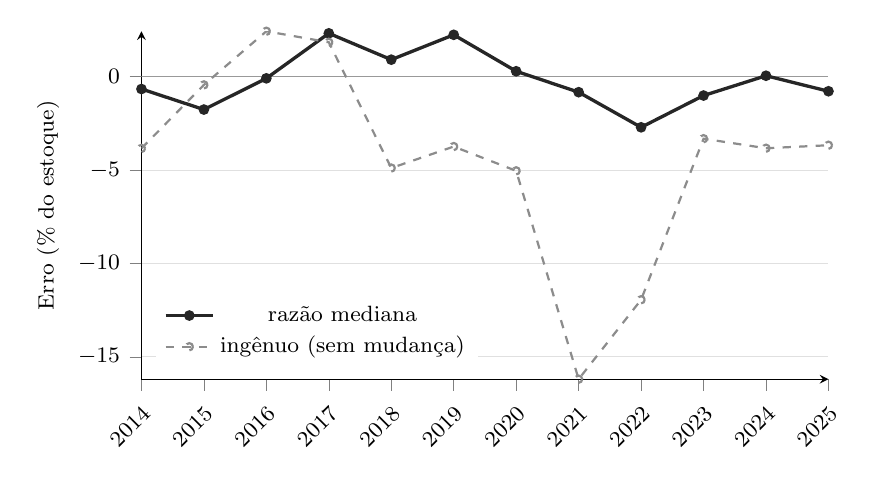
\begin{tikzpicture}
    \begin{axis}[width=\linewidth, height=6.2cm, axis lines=left, tick align=outside,
            ymajorgrids, grid style={black!12}, tick label style={font=\footnotesize},
            label style={font=\footnotesize}, title style={font=\small\bfseries},
            /pgf/number format/use comma, /pgf/number format/1000 sep={.}, width=0.85\textwidth, height=6cm, ylabel={Erro (\% do estoque)},
            xmin=2014, xmax=2025, xtick distance=1,
            x tick label style={/pgf/number format/1000 sep={}, rotate=45, anchor=north east},
            legend style={font=\footnotesize, at={(0.02,0.03)}, anchor=south west, draw=none, fill=white}]
        \addplot[black!40, thin, forget plot] coordinates {(2014,0) (2025,0)};
        \addplot[very thick, black!85, mark=*, mark size=1.3pt] coordinates {(2014,-0.66) (2015,-1.76) (2016,-0.09) (2017,2.32) (2018,0.91) (2019,2.24) (2020,0.29) (2021,-0.83) (2022,-2.71) (2023,-1.01) (2024,0.05) (2025,-0.78)};
        \addlegendentry{razão mediana}
        \addplot[thick, black!45, dashed, mark=o, mark size=1.3pt] coordinates {(2014,-3.84) (2015,-0.44) (2016,2.43) (2017,1.84) (2018,-4.89) (2019,-3.74) (2020,-5.04) (2021,-16.19) (2022,-11.94) (2023,-3.32) (2024,-3.83) (2025,-3.67)};
        \addlegendentry{ingênuo (sem mudança)}
    \end{axis}
    \end{tikzpicture}
    \\[4pt]
    {\footnotesize Erro positivo: o estimador superestimou o estoque. }Fonte: Autoria própria, a partir da camada Gold.
\end{figure}
